
\section{Raggiungibilità ed osservabilità}
Queste due proprietà cercano di studiare in modo qualitativo le potenzialità
dell'ingresso di un certo sistema ISU e la possibilità che offre l'uscita
rispetto alla possibilità di capire cosa accade nel sistema osservando l'uscita.
Le potenzialità dell'ingresso possono influenzare l'evoluzione dello stato,
racchiuso in un sottospazio $X^n$ dell'intero sistema, non è infatti detto che
l'ingresso possa modificare senza vincoli tutte le variabili di stato, questo
fenomeno viene studiato attraverso la proprietà di raggiungibilità.

Si vuole inoltre capire se è possibile ricostruire l'evoluzione interna dello
stato attraverso l'osservazione dell'uscita, in generale non è possibile, si può
ricostruire una parte dello stato e non tutto.

\subsection{Raggiungibilità (LTI)}
Uno stato $\hat{x}$ è raggiungibile se e solo se
$$
\hat{x} \text{ raggiungibile} \Leftrightarrow  \exists \hat{t},
\hat{u}_{[t_0,\hat{t}]} : \left.x_f(\hat{t})\right|_{u=\hat{u}} = \hat{x}
$$
esiste un tempo $\hat{t}$ ed un ingresso $\hat{u}$ tali per cui l'evoluzione
forzata $x_f(\hat{t})$ coincida con lo stato $\hat{x}$.
Questa caratteristica equivale a dire che è possibile pilotare il sistema
mediante l'ingresso in un certo intervallo finito e portarlo proprio nello
stato desiderato.
Un sistema in cui tutti gli stati sono raggiungibili si dirà
\textit{completamente raggiungibile}, si definisce il sottospazio di
raggiungibilità $X_R$ sottoinsieme dello spazio dello stato.
$$
X_R = \{ x\in X^n : x \text{ è raggiungibile}\} \subseteq X^n
$$
Se il sottospazio di raggiungibilità coincide con lo spazio dello stato allora
il sistema nella sua forma ISU è completamente raggiungibile.
La raggiungibilità è fondamentale per un progettista, permette di capire se si
hanno a disposizione i giusti ingressi per il sistema in esame e per
modificarne lo stato.

Si consideri la funzione della risposta forzata dalle formule di Lagrange
$$
x_f(t) = \int_{t_0}^t e^{A(t-t_0)}Bu(\tau) d\tau
$$
Nell'espressione compaiono solo le matrici $A$ e $B$, dunque la proprietà di
raggiungibilità dipende solo da queste due matrici. La matrice $A$ contiene i
modi naturali e le caratteristiche interne al sistema, la matrice $B$ invece
modula l'ingresso e lo lega alla variabile di stato.

Un drone ad esempio è un sistema sottoattuato, non si può controllare
istantaneamente la sua posizione e il suo orientamento ma si possono solo
comandare i motori e quindi la spinta risultante, non si può in alcun modo
applicare una spinta (senza aggiungere ulteriori eliche e dunque variabili di
ingresso) che sia ortogonale al piano del drone.

\subsubsection{Matrice di raggiungibilità}
Permette di studiare la raggiungibilità del sistema, è una matrice a blocchi
per colonna, il primo blocco è la matrice $B$, poi il prodotto di $A\times B$
fino ad $A^{n-1}B$ dove $n$ è la dimensione del sistema (o della matrice $A$)
$$
R=\left(\begin{array}{c|c|c|c|c}
   B & AB & A^2B & \dots & A^{n-1}B
  \end{array}\right)\qquad n\times(n\cdot m )
$$
Uno stato $\hat{x}$ è raggiungibile se e solo se
$$
\hat{x} \text{ raggiungibile} \Leftrightarrow \hat{x} \in X_R =
\text{Immagine}\{R\}
$$
Un sistema è completamente raggiungibile se $X_R$ corrisponde a tutto lo spazio
$X^n$ ma ciò è vero se la matrice $R$ è di ragno pieno.
Per i sistemi con un solo ingresso la matrice diventa quadrata, è sufficiente
assicurarsi che il determinante sia diverso da zero affinchè abbia rango
massimo.

Si consideri il seguente esempio
$$
A = \begin{pmatrix}
     1 & 2 \\
     1 & 2
    \end{pmatrix}
\quad B = \begin{pmatrix}
           1 \\ 1
          \end{pmatrix} \longrightarrow
R=
\begin{array}{c}
B \ AB \\
\left(\begin{array}{c:c}
    1 & 3 \\
    1 & 3
   \end{array}\right)
\end{array}\quad
\rho(R) = 1 < 2
$$
Il sottospazio di raggiungibilità $X_R$ non coincide con tutto lo spazio di
stato, si deve ricavare la base associata alla matrice $R$ estraendo le colonne
linearmente indipendenti, in questo caso è sufficiente usare la prima colonna
$$
\text{Immagine}\{R\} = <\begin{bmatrix}
                         1 \\ 1
                        \end{bmatrix}>
$$
Lo spazio ha dimensione 2 $(n=2)$ mentre la base ha dimensione 1, dunque il
sottospazio di raggiungibilità è la retta passante per l'origine degli assi
dello stato con pendenza unitaria.
Ciò significa che si può fornire al sistema un ingresso qualsiasi ma lo stato
sarà vincolato a muoversi solo lungo la retta $X_R$ ossia tale che $x_1=x_2$
qualunque sia l'ingresso.
La proprietà di raggiungibilità è una proprietà differenziale, non dipende
dalla durata dell'ingresso, se pure si fornisse un ingresso per un tempo
inferiore, al limite infinitesimo, aumentando l'ampiezza dell'ingresso, al
limite impulsivo, si otterrebbe comunque uno stato pari al prodotto $Bu(t)$.

Per capire quali parti dello stato sono raggiungibili e quali non lo sono,
è necessario eseguire una trasformazione di similitudine mediante una matrice,
ci si pone nell'ipotesi $\rho(R) = n_r<n$ altrimenti il sistema sarebbe
completamente raggiungibile, esiste un'intera classe di matrici $T_R$
invertibili
$$
\rho(R) = n_r<n \Rightarrow \exists T_R \text{ invertibile} : x=T_rz
$$
dunque le matrici $A$ e $B$ diventano
$$
A_R = T_R^{-1} A T_R = \begin{pmatrix}
                        A_{11} & A_{12} \\
                        0 & A_{22}
                       \end{pmatrix}
\qquad
B_R = \begin{pmatrix}
       B_1 \\ 0
      \end{pmatrix} = T_R^{-1}B
$$
Si otterranno delle matrici a blocchi triangolari superiori, la matrice
$A_{11}$ di dimensioni $n_r \times n_r$ mentre la $B_1$ sarà $n_r \times m$

La matrice C diventa
$$
C_R = CT_r = \begin{pmatrix}
              C_1 & C_2
             \end{pmatrix}
$$
Il nuovo sistema ISU diventa
$$
\left\{\begin{aligned}
\dot{z} &= A_R z + B_R u \\
y &= C_Rz + Du
\end{aligned}\right.
$$
Si partizione il vettore $z$ chiamando i suoi primi $n_R$ elementi $Z_1$ e i
restanti $n-n_R$ si chiameranno $Z_2$.
$$
z = \begin{pmatrix}
Z_1 \\ Z_2
\end{pmatrix}
$$

Il sistema così partizionato assume la seguente struttura
$$
\left\{\begin{aligned}
\dot{Z}_1 &= A_{11}Z_1 + A_{12} Z_2 + B_1 u\\
\dot{Z}_2 &= A_{22}Z_2\\
y &= C_1Z_1 + C_2 Z_2 +Du
\end{aligned}\right.
$$
Si mostra una rappresentazione grafica del sistema, può essere visto suddiviso
in due sottosistemi, il primo associato alla prima equazione differenziale e il
secondo alla seconda.
Per il primo sottosistema la matrice $A_{11}$ coincide alla sua matrice della
dinamica, dipende dallo stato $Z_1$ mentre la matrice $A_{12}$ rappresenta la
mutua relazione tra il sottosistema $Z_1$ e l'ingresso $Z_2$ fornito dal
rispettivo sottosistema, dunque $Z_2$ può essere considerato come un ingresso
per il sottosistema $Z_1$.
Il sottosistema $Z_2$ è autonomo, non ha ingressi, dunque non è raggiungibile.
\begin{figure}[h]
 \centering
 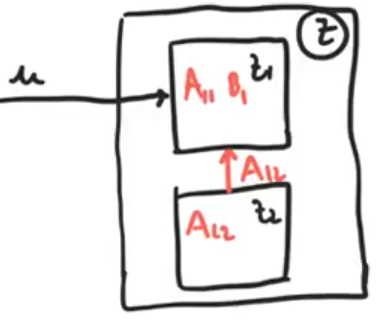
\includegraphics[width=\picwid]{sistema_raggiungibile}
\end{figure}

Si dimostra che la coppia $(A_{11},B_1)$ è completamente raggiungibile
$$
\rho({R}) = \rho\left(B_R,\ A_RB_R\ \dots\ A_R^{n-1}B_R\right) = \rho
\begin{pmatrix}
B_1 & A_{11}B_1 & \ldots & A_{11}^{n-1}B_1\\
 0  &     0     &        &   0
\end{pmatrix}
\stackrel{\text{ipotesi}}{=}n_R
$$

La prima riga della matrice $R$ contiene $n_R$ righe per costruzione, dato che
il rango è massimo allora tutte le colonne saranno linearmente indipendenti tra
loro ma queste colonne formano proprio la matrice di raggiungibilità del
sottosistema 1, dunque esso è completamente raggiungibile.

La matrice della dinamica è triangolare alta, dunque i suoi autovalori sono gli
autovalori dei blocchi sulla diagonale, ossia di $A_{11}$ e $A_{22}$ ma i primi
appartengono alla parte raggiungibile, quelli di $A_{22}$ no.

La matrice $T_R$ deve essere invertibile, si costruisce nel seguente modo: si
inseriscono $n_R$ colonne linearmente indipendenti tali che siano una base di
$X_R$ possono essere prese dalla matrice di raggiungibilità $R$ ed
eventualmente combinarle affinché siano ancora una base, si completa la matrice
$T_R$ con $(n-n_R)$ colonne arbitrarie, rispettando sempre il
vincolo $\text{det}(T_R)\neq 0$.

Si considerino le matrici dell'esempio precedente
$$
A=\begin{pmatrix}
1 & 2 \\
1 & 2
\end{pmatrix} \quad
B=\begin{pmatrix}
1 \\ 1
\end{pmatrix} \quad
X_R = <\begin{bmatrix}
1 \\ 1
\end{bmatrix}> \quad
T_R = \begin{pmatrix}
1 & 1 \\
1 & -1
\end{pmatrix}$$
Si calcola la matrice di trasformazione e le matrici $A_R$ e $B_R$, si ricorda
che in questo specifico caso il valore $A_{22}$ è zero perché è uno
degli autovalori di $A$, non è un motivo strutturale della matrice $A_R$ come
lo zero in posizione (2,1).
$$
A_R = T_R^{-1}AT_R = \begin{pmatrix}
A_{11} & A_{12} \\
0 & A_{22}
\end{pmatrix}=
\begin{pmatrix}
3 & -1 \\
0 & 0
\end{pmatrix}\quad
B_R = T_R^{-1}B = \begin{pmatrix}
1 \\ 0
\end{pmatrix}
$$
$\lambda_1=3$ è l'autovalore della parte raggiungibile, $\lambda_2=0$ è non
raggiungibile.

\subsubsection{Influenza sull'uscita dalla raggiungibilità}
La risposta di un sistema è la convoluzione della funzione di trasferimento e
l'ingresso
$$
w(t) = Ce^{At}B = CT_RT_R^{-1}e^{At}T_RT_R^{-1}B
= CT_Re^{T_R^{-1}AT_Rt}T_R^{-1}B = C_Re^{A_Rt}B_R
$$
Il legame ingresso-uscita non dipende dunque dalla forma di rappresentazione
dello stato. Ricordando la definizione della matrice esponenziale
$$\begin{aligned}
w(t) &= (C_1\ C_2) e^{\begin{pmatrix}
A_{11} & A_{12} \\
0 & A_{22}
\end{pmatrix}t}\begin{pmatrix}
B_1 \\ 0
\end{pmatrix} =
(C_1 \ C_2) \sum_{k=0}^{+\infty} \frac{t^k}{k!}\begin{pmatrix}
A_{11} & A_{12} \\
0 & A_{22}
\end{pmatrix}^k
\begin{pmatrix}
B_1 \\ 0
\end{pmatrix} = \\
&= (C_1 \ C_2) \sum_{k=0}^{+\infty} \frac{t^k}{k!}
\begin{pmatrix}
A_{11}^k & * \\
0 & A_{22}^k
\end{pmatrix}
\begin{pmatrix}
B_1 \\ 0
\end{pmatrix} =
(C_1 \ C_2) \sum_{k=0}^{+\infty} \frac{t^k}{k!}
\begin{pmatrix}
A_{11}^k B_1 \\ 0
\end{pmatrix} = \\
&= C_1\left(\sum_{k=0}^{+\infty} \frac{t^k}{k!}
A_{11}^k\right)B_1 = C_1 e^{A_{11}t}B_1 = w_1(t)
\end{aligned}
$$
La seconda colonna della matrice esponenziale viene moltiplicata per 0, non è
necessario calcolare il termine $*$.
Si è ricavato che la risposta all'impulso si può calcolare più rapidamente se
si usa una matrice più piccola $(A_{11}=3)$ nel caso in cui il sistema non sia
completamente raggiungibile. Si è dimostrato inoltre che la risposta
all'impulso dipende solo dalla parte raggiungibile del sistema.
Eseguendo la trasformata di Laplace si ottiene la funzione di trasferimento e
si ricavano i poli rispettivi alla parte raggiungibile.

\subsection{Osservabilità}
Definisce la possibilità di capire l'evoluzione interna di uno stato osservando
l'uscita.
Si fornisce la definizione di cosa \textit{non} è osservabile dato che ha una
struttura di spazio vettoriale mentre l'osservabilità è uno spazio
algebrico.

Si definiscono due stati inosservabili, o meglio \textit{indistinguibili}.
Si sottopone un sistema ad un ingresso $u$ e si osserva l'uscita $y$, lo stato
avrà un'evoluzione nel tempo, la $y=Cx+Du$.
Lo stesso sistema partendo da uno stato differente $X_0''$, sottoposto allo
stesso ingresso potrebbe raggiungere la stessa uscita. In tal caso i due stati
si direbbero \textit{indistinguibili} se le due uscite coincidono.

Si riportano le formule di Lagrange in tale condizione
$$
Ce^{A(t-t_0)}x_0' + \cancel{\int_{t_0}^t e^{A(t-\tau)}Bu(\tau)d\tau} =
Ce^{A(t-t_0)}x_0'' + \cancel{\int_{t_0}^t e^{A(t-\tau)}Bu(\tau)d\tau}
$$
La inosservabilità degli stati non dipende dagli ingressi ma solo
dall'evoluzione libera.
$$
Ce^{A(t-t_0)}(x_0'-x_0'') = 0 = \left.y_l(t)
\right|_{x_0=(x_0'-x_0'')}
$$
Lo stato $x_0$ definito come differenza tra gli altri due potrebbe portare ad
avere un'uscita libera nulla, nonostante il sistema evolva necessariamente al
suo interno. Si dirà il generico stato $\overline{x}$
inosservabile se e solo se è indistinguibile dall'evoluzione libera che parte
dallo stato nullo
$$
y_l(t) = Ce^{A(t-t_0)}\overline{x}=0
$$

Si vuole studiare se un sistema ISU ha stati inosservabili, mediante l'ausilio
della matrice di osservabilità.
Si definisce lo spazio di inosservabilità
$$
X_I \stackrel{\text{def}}{=}\{x\in X^n:x\text{ è inosservabile}\}
$$
La matrice di osservabilità riempita a blocchi per righe invece
$$
O = \begin{pmatrix}
C \\ CA \\ \vdots \\CA^{n-1}
\end{pmatrix} \quad (p\cdot n) \times n
$$
Un vettore $\overline{X}$ è inosservabile se
$$
\overline{x} \text{ inosservabile} \Leftrightarrow
\overline{x} \in X_I = \text{Ker}\{O\}
$$
Se lo spazio di inosservabilità è vuoto
$$
X_I = \text{\O{}} \Leftrightarrow \text{Sistema ISU $(A,C)$ è completamente
osservabile}
$$

\newpage
\subsubsection{Esempio numerico}
Sia il seguente sistema
$$
A= \begin{pmatrix}
1 & 2 \\
2 & 1
\end{pmatrix}\quad
C= \begin{pmatrix}
1 & 1
\end{pmatrix} \longrightarrow
O = \begin{pmatrix}
C \\ CA
\end{pmatrix} =
\begin{pmatrix}
1 & 1 \\
3 & 3
\end{pmatrix}
$$
La dimensione del Kernel di $O$ è pari alla sua dimensione $n$ meno il suo
rango, se la matrice $O$ fosse di rango pieno, la dimensione di inosservabilità
sarebbe vuota.
$$
\rho(O) = \rho
\begin{pmatrix}
1 & 1 \\
3 & 3
\end{pmatrix}
=1 < 2$$

$$
X_I = \text{Ker}\{O\} = \text{Ker}\begin{pmatrix}
1 & 1\\
3 & 3
\end{pmatrix} =
\left\{x\in\mathbb{R}^2:\begin{pmatrix}
1 & 1 \\ 3 & 3
\end{pmatrix}x=0\right\} = <\begin{bmatrix}
1 \\ -1
\end{bmatrix}>
$$
Rappresentando graficamente lo spazio di inosservabilità si ottiene una retta
passante per l'origine e il punto $(1,-1)$, ossia a pendenza -1. Qualunque
stato iniziale che giace su questa retta è inosservabile.

\subsubsection{Sottosistemi osservabili e non osservabili}
Ricapitolando
$$
X_I \subseteq X^n \text{ spazio vettoriale}
$$
$$
\rho(O) = n \Leftrightarrow X_I = \text{\O{}} \Leftrightarrow
\text{Sistema (coppia $(A,C)$) completamente osservabile }
$$
Se il numero di uscite $p=1$ è sufficiente verificare che il determinante di
$O$ sia diverso da zero affinché il sistema sia completamente osservabile.

Se
$$
\rho(O) = n_o < n \quad \text{dim}\left\{
\text{Ker}\{O\}
\right\} = n -n_o > 0
$$
allora
$$
\exists T_o \text{ invertibile}: x=T_oz:
\left\{\begin{aligned}
\dot{z} &= A_oz + B_ou \\
y &= C_oz +Du
\end{aligned}\right.
$$
La struttura delle matrici trasformate è triangolare bassa
$$
A_o = T^{-1}_oAT_o = \begin{pmatrix}
A_{11} & 0 \\
A_{21} & A_{22}
\end{pmatrix} \quad
C_o = CT_o = (C_1\ 0) \quad
B_o = T_0^{-1} B = \begin{pmatrix}
B_1 \\ B_2
\end{pmatrix}
$$
$A_{11} = (n_o\times n_o)$, $C_1 = (p\times n_o)$ mentre la matrice $B_o$ non
ha alcuna struttura particolare ma si suddividono le sue prime $n_o$ righe in
$B_1$.

Si suddivide il vettore di stato $z$ in cui $Z_1$ si trovano le prime
$n_o$ righe e $Z_2$ le rimanenti $(n-n_o)$, il sistema ISU diventa
$$
\left\{\begin{aligned}
\dot{z}_1 & = A_{11} Z_1 + B_1u \\
\dot{z}_2 &= A_{21} Z_1 + A_{22} Z_2 +B_2 u \\
y & = C_1Z_1
\end{aligned}\right.
$$

\newpage
Una rappresentazione grafica del sistema è la seguente
\begin{figure}[h]
\centering
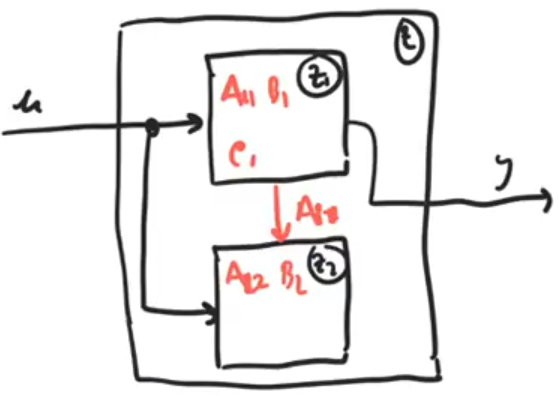
\includegraphics[width=\picwid]{sistema_osservabile}
\end{figure}
L'uscita non ha influenze dirette o indirette dal sotto-sistema $Z_2$.
Se si considera il rango della matrice di osservabilità
$$
\rho(O) = \rho \begin{pmatrix}
C_o\\C_oA_o \\ \vdots \\ C_oA^{n-1}_o
\end{pmatrix} =\rho
\begin{pmatrix}
C_1 & 0 \\
C_1 A_{11} & 0\\
\vdots & \vdots \\
C_1A_{11}^{n-1} & 0
\end{pmatrix}\stackrel{\text{Hp.}}{=} n_o
$$
La prima colonna è formata da $n_o$ elementi, dunque saranno necessariamente
indipendenti tra loro, possono essere però associati alla matrice di
osservabilità del primo sottosistema $O_1$, dunque $\rho(O_1) = n_o$ la matrice
$(A_{11},C_1)$ è completamente osservabile mentre la matrice $A_{22}$
corrisponde alla parte inosservabile.

Essendo $A_o$ triangolare, i suoi autovalori saranno gli autovalori delle
matrici $A_{11}$ e $A_{22}$ sulla diagonale, $A_{11}$ conterrà gli autovalori
della parte osservabile, viceversa $A_{22}$ quelli della parte non osservabile.

La matrice $T_o$ si costruisce nel seguente modo: si posiziona una base dello
spazio inosservabile $X_I$ nelle ultime $n_o$ colonne, si completa la matrice
con le restanti $(n-n_o)$ colonne affinché il determinante di $T_o$ sia sempre
diverso da zero.
Ad esempio
$$
A= \begin{pmatrix}
1 & 2 \\ 2 & 1
\end{pmatrix}\quad
C = (1\ 1)\rightarrow
X_I = <\begin{bmatrix}
1 \\ -1
\end{bmatrix}>
\rightarrow
T_o = \begin{pmatrix}
1 & 1 \\
1 & -1
\end{pmatrix}
$$
Dunque la matrice $A_o$
$$
A_o = T_o^{-1} A T_o = \begin{pmatrix}
3 & 0 \\
0 & -1
\end{pmatrix}
$$
3 è l'autovalore osservabile, -1 è quello non osservabile, lo 0 in posizione
(1,2) è strutturale, quello in (2,1) è capitato.
$$
C_0 = (1\ 0)
$$

\newpage
Si analizza la risposta all'impulso
$$\begin{aligned}
w(t) &= Ce^{At}B = CT_oT_o^{-1}e^{At} T_oT_o^{-1}B = C_o e^{A_ot}B_o = (C_1\ 0)
e^{\begin{pmatrix}
A_{11} & 0 \\
A_{21} & A_{22}
\end{pmatrix}t
}\begin{pmatrix}
B_1 \\ B_2
\end{pmatrix} = \\
&=C_1 e ^{A_{11}t}B_1 = w_1(t)
\end{aligned}
$$
La risposta all'impulso dipende solo dalla parte osservabile del sistema.

Se un sistema non è completamente raggiungibile e osservabile, avrà una
risposta all'impulso molto più piccola dimensionalmente dell'intero sistema.

\subsubsection{Test di Popov-Belevitch-Hautus (PBH)}
Un sistema è completamente raggiungibile se e solo se
$$
\rho(A-\lambda I \ B) = n\qquad \forall i = 1,\dots, n
$$
Il sistema è completamente osservabile se e solo se
$$
\rho \begin{pmatrix}
A-\lambda_i I \\
C
\end{pmatrix} = n \qquad\forall i =1,\dots,n
$$
Questi due test devono essere eseguiti per ogni autovalore $\lambda_i$.
